% Created by tikzDevice version 0.12.3.1 on 2021-04-14 08:52:34
% !TEX encoding = UTF-8 Unicode
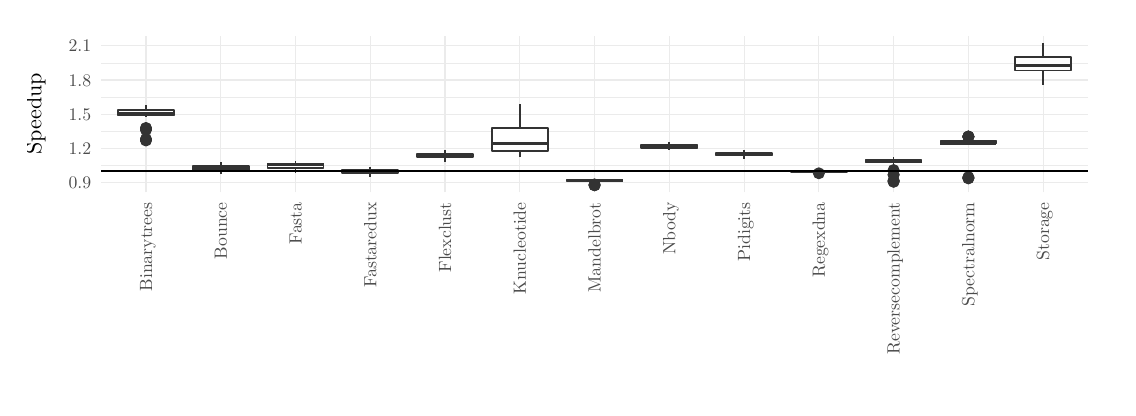
\begin{tikzpicture}[x=1pt,y=1pt]
\definecolor{fillColor}{RGB}{255,255,255}
\path[use as bounding box,fill=fillColor,fill opacity=0.00] (0,0) rectangle (390.26,130.09);
\begin{scope}
\path[clip] ( 26.53, 70.57) rectangle (383.14,127.24);
\definecolor{drawColor}{gray}{0.92}

\path[draw=drawColor,line width= 0.2pt,line join=round] ( 26.53, 80.24) --
	(383.14, 80.24);

\path[draw=drawColor,line width= 0.2pt,line join=round] ( 26.53, 92.62) --
	(383.14, 92.62);

\path[draw=drawColor,line width= 0.2pt,line join=round] ( 26.53,105.00) --
	(383.14,105.00);

\path[draw=drawColor,line width= 0.2pt,line join=round] ( 26.53,117.38) --
	(383.14,117.38);

\path[draw=drawColor,line width= 0.4pt,line join=round] ( 26.53, 74.05) --
	(383.14, 74.05);

\path[draw=drawColor,line width= 0.4pt,line join=round] ( 26.53, 86.43) --
	(383.14, 86.43);

\path[draw=drawColor,line width= 0.4pt,line join=round] ( 26.53, 98.81) --
	(383.14, 98.81);

\path[draw=drawColor,line width= 0.4pt,line join=round] ( 26.53,111.19) --
	(383.14,111.19);

\path[draw=drawColor,line width= 0.4pt,line join=round] ( 26.53,123.57) --
	(383.14,123.57);

\path[draw=drawColor,line width= 0.4pt,line join=round] ( 42.74, 70.57) --
	( 42.74,127.24);

\path[draw=drawColor,line width= 0.4pt,line join=round] ( 69.76, 70.57) --
	( 69.76,127.24);

\path[draw=drawColor,line width= 0.4pt,line join=round] ( 96.77, 70.57) --
	( 96.77,127.24);

\path[draw=drawColor,line width= 0.4pt,line join=round] (123.79, 70.57) --
	(123.79,127.24);

\path[draw=drawColor,line width= 0.4pt,line join=round] (150.81, 70.57) --
	(150.81,127.24);

\path[draw=drawColor,line width= 0.4pt,line join=round] (177.82, 70.57) --
	(177.82,127.24);

\path[draw=drawColor,line width= 0.4pt,line join=round] (204.84, 70.57) --
	(204.84,127.24);

\path[draw=drawColor,line width= 0.4pt,line join=round] (231.85, 70.57) --
	(231.85,127.24);

\path[draw=drawColor,line width= 0.4pt,line join=round] (258.87, 70.57) --
	(258.87,127.24);

\path[draw=drawColor,line width= 0.4pt,line join=round] (285.89, 70.57) --
	(285.89,127.24);

\path[draw=drawColor,line width= 0.4pt,line join=round] (312.90, 70.57) --
	(312.90,127.24);

\path[draw=drawColor,line width= 0.4pt,line join=round] (339.92, 70.57) --
	(339.92,127.24);

\path[draw=drawColor,line width= 0.4pt,line join=round] (366.94, 70.57) --
	(366.94,127.24);
\definecolor{drawColor}{gray}{0.20}
\definecolor{fillColor}{gray}{0.20}

\path[draw=drawColor,line width= 0.4pt,line join=round,line cap=round,fill=fillColor] ( 42.74, 93.85) circle (  1.96);

\path[draw=drawColor,line width= 0.4pt,line join=round,line cap=round,fill=fillColor] ( 42.74, 93.70) circle (  1.96);

\path[draw=drawColor,line width= 0.4pt,line join=round,line cap=round,fill=fillColor] ( 42.74, 93.42) circle (  1.96);

\path[draw=drawColor,line width= 0.4pt,line join=round,line cap=round,fill=fillColor] ( 42.74, 93.13) circle (  1.96);

\path[draw=drawColor,line width= 0.4pt,line join=round,line cap=round,fill=fillColor] ( 42.74, 89.83) circle (  1.96);

\path[draw=drawColor,line width= 0.4pt,line join=round,line cap=round,fill=fillColor] ( 42.74, 89.63) circle (  1.96);

\path[draw=drawColor,line width= 0.4pt,line join=round,line cap=round,fill=fillColor] ( 42.74, 89.57) circle (  1.96);

\path[draw=drawColor,line width= 0.4pt,line join=round,line cap=round,fill=fillColor] ( 42.74, 89.32) circle (  1.96);

\path[draw=drawColor,line width= 0.6pt,line join=round] ( 42.74,100.35) -- ( 42.74,102.14);

\path[draw=drawColor,line width= 0.6pt,line join=round] ( 42.74, 98.39) -- ( 42.74, 97.69);
\definecolor{fillColor}{RGB}{255,255,255}

\path[draw=drawColor,line width= 0.6pt,line join=round,line cap=round,fill=fillColor] ( 32.61,100.35) --
	( 32.61, 98.39) --
	( 52.87, 98.39) --
	( 52.87,100.35) --
	( 32.61,100.35) --
	cycle;

\path[draw=drawColor,line width= 1.1pt,line join=round] ( 32.61, 99.16) -- ( 52.87, 99.16);

\path[draw=drawColor,line width= 0.6pt,line join=round] ( 69.76, 80.19) -- ( 69.76, 81.55);

\path[draw=drawColor,line width= 0.6pt,line join=round] ( 69.76, 78.72) -- ( 69.76, 77.10);

\path[draw=drawColor,line width= 0.6pt,line join=round,line cap=round,fill=fillColor] ( 59.63, 80.19) --
	( 59.63, 78.72) --
	( 79.89, 78.72) --
	( 79.89, 80.19) --
	( 59.63, 80.19) --
	cycle;

\path[draw=drawColor,line width= 1.1pt,line join=round] ( 59.63, 79.32) -- ( 79.89, 79.32);

\path[draw=drawColor,line width= 0.6pt,line join=round] ( 96.77, 81.04) -- ( 96.77, 81.80);

\path[draw=drawColor,line width= 0.6pt,line join=round] ( 96.77, 79.33) -- ( 96.77, 77.55);

\path[draw=drawColor,line width= 0.6pt,line join=round,line cap=round,fill=fillColor] ( 86.64, 81.04) --
	( 86.64, 79.33) --
	(106.90, 79.33) --
	(106.90, 81.04) --
	( 86.64, 81.04) --
	cycle;

\path[draw=drawColor,line width= 1.1pt,line join=round] ( 86.64, 80.81) -- (106.90, 80.81);

\path[draw=drawColor,line width= 0.6pt,line join=round] (123.79, 78.55) -- (123.79, 79.68);

\path[draw=drawColor,line width= 0.6pt,line join=round] (123.79, 77.48) -- (123.79, 76.09);

\path[draw=drawColor,line width= 0.6pt,line join=round,line cap=round,fill=fillColor] (113.66, 78.55) --
	(113.66, 77.48) --
	(133.92, 77.48) --
	(133.92, 78.55) --
	(113.66, 78.55) --
	cycle;

\path[draw=drawColor,line width= 1.1pt,line join=round] (113.66, 78.09) -- (133.92, 78.09);

\path[draw=drawColor,line width= 0.6pt,line join=round] (150.81, 84.47) -- (150.81, 85.77);

\path[draw=drawColor,line width= 0.6pt,line join=round] (150.81, 83.33) -- (150.81, 81.72);

\path[draw=drawColor,line width= 0.6pt,line join=round,line cap=round,fill=fillColor] (140.67, 84.47) --
	(140.67, 83.33) --
	(160.94, 83.33) --
	(160.94, 84.47) --
	(140.67, 84.47) --
	cycle;

\path[draw=drawColor,line width= 1.1pt,line join=round] (140.67, 83.74) -- (160.94, 83.74);

\path[draw=drawColor,line width= 0.6pt,line join=round] (177.82, 93.95) -- (177.82,102.37);

\path[draw=drawColor,line width= 0.6pt,line join=round] (177.82, 85.44) -- (177.82, 83.22);

\path[draw=drawColor,line width= 0.6pt,line join=round,line cap=round,fill=fillColor] (167.69, 93.95) --
	(167.69, 85.44) --
	(187.95, 85.44) --
	(187.95, 93.95) --
	(167.69, 93.95) --
	cycle;

\path[draw=drawColor,line width= 1.1pt,line join=round] (167.69, 88.20) -- (187.95, 88.20);
\definecolor{fillColor}{gray}{0.20}

\path[draw=drawColor,line width= 0.4pt,line join=round,line cap=round,fill=fillColor] (204.84, 73.46) circle (  1.96);

\path[draw=drawColor,line width= 0.4pt,line join=round,line cap=round,fill=fillColor] (204.84, 73.18) circle (  1.96);

\path[draw=drawColor,line width= 0.4pt,line join=round,line cap=round,fill=fillColor] (204.84, 73.16) circle (  1.96);

\path[draw=drawColor,line width= 0.4pt,line join=round,line cap=round,fill=fillColor] (204.84, 73.15) circle (  1.96);

\path[draw=drawColor,line width= 0.6pt,line join=round] (204.84, 74.99) -- (204.84, 75.22);

\path[draw=drawColor,line width= 0.6pt,line join=round] (204.84, 74.68) -- (204.84, 74.38);
\definecolor{fillColor}{RGB}{255,255,255}

\path[draw=drawColor,line width= 0.6pt,line join=round,line cap=round,fill=fillColor] (194.71, 74.99) --
	(194.71, 74.68) --
	(214.97, 74.68) --
	(214.97, 74.99) --
	(194.71, 74.99) --
	cycle;

\path[draw=drawColor,line width= 1.1pt,line join=round] (194.71, 74.90) -- (214.97, 74.90);

\path[draw=drawColor,line width= 0.6pt,line join=round] (231.85, 87.76) -- (231.85, 88.67);

\path[draw=drawColor,line width= 0.6pt,line join=round] (231.85, 86.71) -- (231.85, 85.90);

\path[draw=drawColor,line width= 0.6pt,line join=round,line cap=round,fill=fillColor] (221.72, 87.76) --
	(221.72, 86.71) --
	(241.99, 86.71) --
	(241.99, 87.76) --
	(221.72, 87.76) --
	cycle;

\path[draw=drawColor,line width= 1.1pt,line join=round] (221.72, 86.93) -- (241.99, 86.93);

\path[draw=drawColor,line width= 0.6pt,line join=round] (258.87, 84.86) -- (258.87, 86.04);

\path[draw=drawColor,line width= 0.6pt,line join=round] (258.87, 83.94) -- (258.87, 82.74);

\path[draw=drawColor,line width= 0.6pt,line join=round,line cap=round,fill=fillColor] (248.74, 84.86) --
	(248.74, 83.94) --
	(269.00, 83.94) --
	(269.00, 84.86) --
	(248.74, 84.86) --
	cycle;

\path[draw=drawColor,line width= 1.1pt,line join=round] (248.74, 84.39) -- (269.00, 84.39);
\definecolor{fillColor}{gray}{0.20}

\path[draw=drawColor,line width= 0.4pt,line join=round,line cap=round,fill=fillColor] (285.89, 77.47) circle (  1.96);

\path[draw=drawColor,line width= 0.6pt,line join=round] (285.89, 78.34) -- (285.89, 78.45);

\path[draw=drawColor,line width= 0.6pt,line join=round] (285.89, 78.04) -- (285.89, 77.67);
\definecolor{fillColor}{RGB}{255,255,255}

\path[draw=drawColor,line width= 0.6pt,line join=round,line cap=round,fill=fillColor] (275.76, 78.34) --
	(275.76, 78.04) --
	(296.02, 78.04) --
	(296.02, 78.34) --
	(275.76, 78.34) --
	cycle;

\path[draw=drawColor,line width= 1.1pt,line join=round] (275.76, 78.27) -- (296.02, 78.27);
\definecolor{fillColor}{gray}{0.20}

\path[draw=drawColor,line width= 0.4pt,line join=round,line cap=round,fill=fillColor] (312.90, 78.65) circle (  1.96);

\path[draw=drawColor,line width= 0.4pt,line join=round,line cap=round,fill=fillColor] (312.90, 77.01) circle (  1.96);

\path[draw=drawColor,line width= 0.4pt,line join=round,line cap=round,fill=fillColor] (312.90, 76.89) circle (  1.96);

\path[draw=drawColor,line width= 0.4pt,line join=round,line cap=round,fill=fillColor] (312.90, 74.87) circle (  1.96);

\path[draw=drawColor,line width= 0.4pt,line join=round,line cap=round,fill=fillColor] (312.90, 74.80) circle (  1.96);

\path[draw=drawColor,line width= 0.4pt,line join=round,line cap=round,fill=fillColor] (312.90, 74.47) circle (  1.96);

\path[draw=drawColor,line width= 0.4pt,line join=round,line cap=round,fill=fillColor] (312.90, 74.40) circle (  1.96);

\path[draw=drawColor,line width= 0.6pt,line join=round] (312.90, 82.32) -- (312.90, 83.46);

\path[draw=drawColor,line width= 0.6pt,line join=round] (312.90, 81.41) -- (312.90, 80.94);
\definecolor{fillColor}{RGB}{255,255,255}

\path[draw=drawColor,line width= 0.6pt,line join=round,line cap=round,fill=fillColor] (302.77, 82.32) --
	(302.77, 81.41) --
	(323.03, 81.41) --
	(323.03, 82.32) --
	(302.77, 82.32) --
	cycle;

\path[draw=drawColor,line width= 1.1pt,line join=round] (302.77, 81.72) -- (323.03, 81.72);
\definecolor{fillColor}{gray}{0.20}

\path[draw=drawColor,line width= 0.4pt,line join=round,line cap=round,fill=fillColor] (339.92, 90.73) circle (  1.96);

\path[draw=drawColor,line width= 0.4pt,line join=round,line cap=round,fill=fillColor] (339.92, 90.73) circle (  1.96);

\path[draw=drawColor,line width= 0.4pt,line join=round,line cap=round,fill=fillColor] (339.92, 90.71) circle (  1.96);

\path[draw=drawColor,line width= 0.4pt,line join=round,line cap=round,fill=fillColor] (339.92, 90.70) circle (  1.96);

\path[draw=drawColor,line width= 0.4pt,line join=round,line cap=round,fill=fillColor] (339.92, 90.67) circle (  1.96);

\path[draw=drawColor,line width= 0.4pt,line join=round,line cap=round,fill=fillColor] (339.92, 76.10) circle (  1.96);

\path[draw=drawColor,line width= 0.4pt,line join=round,line cap=round,fill=fillColor] (339.92, 75.83) circle (  1.96);

\path[draw=drawColor,line width= 0.4pt,line join=round,line cap=round,fill=fillColor] (339.92, 75.71) circle (  1.96);

\path[draw=drawColor,line width= 0.4pt,line join=round,line cap=round,fill=fillColor] (339.92, 75.64) circle (  1.96);

\path[draw=drawColor,line width= 0.6pt,line join=round] (339.92, 89.14) -- (339.92, 90.19);

\path[draw=drawColor,line width= 0.6pt,line join=round] (339.92, 88.20) -- (339.92, 88.02);
\definecolor{fillColor}{RGB}{255,255,255}

\path[draw=drawColor,line width= 0.6pt,line join=round,line cap=round,fill=fillColor] (329.79, 89.14) --
	(329.79, 88.20) --
	(350.05, 88.20) --
	(350.05, 89.14) --
	(329.79, 89.14) --
	cycle;

\path[draw=drawColor,line width= 1.1pt,line join=round] (329.79, 88.34) -- (350.05, 88.34);

\path[draw=drawColor,line width= 0.6pt,line join=round] (366.94,119.57) -- (366.94,124.66);

\path[draw=drawColor,line width= 0.6pt,line join=round] (366.94,114.57) -- (366.94,109.44);

\path[draw=drawColor,line width= 0.6pt,line join=round,line cap=round,fill=fillColor] (356.80,119.57) --
	(356.80,114.57) --
	(377.07,114.57) --
	(377.07,119.57) --
	(356.80,119.57) --
	cycle;

\path[draw=drawColor,line width= 1.1pt,line join=round] (356.80,116.26) -- (377.07,116.26);
\definecolor{drawColor}{RGB}{0,0,0}

\path[draw=drawColor,line width= 0.6pt,line join=round] ( 26.53, 78.18) -- (383.14, 78.18);
\end{scope}
\begin{scope}
\path[clip] (  0.00,  0.00) rectangle (390.26,130.09);
\definecolor{drawColor}{gray}{0.30}

\node[text=drawColor,anchor=base east,inner sep=0pt, outer sep=0pt, scale=  0.64] at ( 22.93, 71.85) {0.9};

\node[text=drawColor,anchor=base east,inner sep=0pt, outer sep=0pt, scale=  0.64] at ( 22.93, 84.23) {1.2};

\node[text=drawColor,anchor=base east,inner sep=0pt, outer sep=0pt, scale=  0.64] at ( 22.93, 96.61) {1.5};

\node[text=drawColor,anchor=base east,inner sep=0pt, outer sep=0pt, scale=  0.64] at ( 22.93,108.99) {1.8};

\node[text=drawColor,anchor=base east,inner sep=0pt, outer sep=0pt, scale=  0.64] at ( 22.93,121.37) {2.1};
\end{scope}
\begin{scope}
\path[clip] (  0.00,  0.00) rectangle (390.26,130.09);
\definecolor{drawColor}{gray}{0.30}

\node[text=drawColor,rotate= 90.00,anchor=base east,inner sep=0pt, outer sep=0pt, scale=  0.64] at ( 44.94, 66.97) {Binarytrees};

\node[text=drawColor,rotate= 90.00,anchor=base east,inner sep=0pt, outer sep=0pt, scale=  0.64] at ( 71.96, 66.97) {Bounce};

\node[text=drawColor,rotate= 90.00,anchor=base east,inner sep=0pt, outer sep=0pt, scale=  0.64] at ( 98.98, 66.97) {Fasta};

\node[text=drawColor,rotate= 90.00,anchor=base east,inner sep=0pt, outer sep=0pt, scale=  0.64] at (125.99, 66.97) {Fastaredux};

\node[text=drawColor,rotate= 90.00,anchor=base east,inner sep=0pt, outer sep=0pt, scale=  0.64] at (153.01, 66.97) {Flexclust};

\node[text=drawColor,rotate= 90.00,anchor=base east,inner sep=0pt, outer sep=0pt, scale=  0.64] at (180.03, 66.97) {Knucleotide};

\node[text=drawColor,rotate= 90.00,anchor=base east,inner sep=0pt, outer sep=0pt, scale=  0.64] at (207.04, 66.97) {Mandelbrot};

\node[text=drawColor,rotate= 90.00,anchor=base east,inner sep=0pt, outer sep=0pt, scale=  0.64] at (234.06, 66.97) {Nbody};

\node[text=drawColor,rotate= 90.00,anchor=base east,inner sep=0pt, outer sep=0pt, scale=  0.64] at (261.07, 66.97) {Pidigits};

\node[text=drawColor,rotate= 90.00,anchor=base east,inner sep=0pt, outer sep=0pt, scale=  0.64] at (288.09, 66.97) {Regexdna};

\node[text=drawColor,rotate= 90.00,anchor=base east,inner sep=0pt, outer sep=0pt, scale=  0.64] at (315.11, 66.97) {Reversecomplement};

\node[text=drawColor,rotate= 90.00,anchor=base east,inner sep=0pt, outer sep=0pt, scale=  0.64] at (342.12, 66.97) {Spectralnorm};

\node[text=drawColor,rotate= 90.00,anchor=base east,inner sep=0pt, outer sep=0pt, scale=  0.64] at (369.14, 66.97) {Storage};
\end{scope}
\begin{scope}
\path[clip] (  0.00,  0.00) rectangle (390.26,130.09);
\definecolor{drawColor}{RGB}{0,0,0}

\node[text=drawColor,rotate= 90.00,anchor=base,inner sep=0pt, outer sep=0pt, scale=  0.80] at (  4.98, 98.91) {Speedup};
\end{scope}
\end{tikzpicture}
